\section{Analysis of the Evolution of a Single Atom}
  \label{sec:simultons_analysis}

    In order to understand the steep, early response in the \textsc{cw} probe
    signal observed in the experiment and matched in the numerical simulations, we
    turn in this section from the fields to focus on the evolution of the density
    matrix of a single atom as it is addressed by the probe and subsequently
    disturbed by the coupling pulse.

    As discussed in appendix \ref{apx:qu_dyn}, the density matrix $\rho$ is used
    to describe the state of an open quantum system such as an atom interacting
    both with coherent fields and with a stochastically modelled environment. We
    follow the evolution of $\rho$ using the Lindblad master equation
    (\ref{eqn:lindblad_apx}).

    The Hamiltonian for the V-type atom was given in equation
    (\ref{eqn:vee_hamiltonian}). In the case of the pulsed coupling scheme, at the
    front of the medium we have input time-dependent fields $\Omega_p(t)$ and
    $\Omega_c(t)$ and thus a time-dependent Hamiltonian
    $\mathcal{H}_\mathrm{V}(t)$. We can solve the the Lindblad equation
    numerically given an initial condition.

    We imagine the \textsc{cw} probe having plenty of time to equilibrate before
    the pulse, so we first find the steady state solution with the probe on and
    the coupling pulse off. This steady state constitutes the initial condition.

    \begin{figure}
    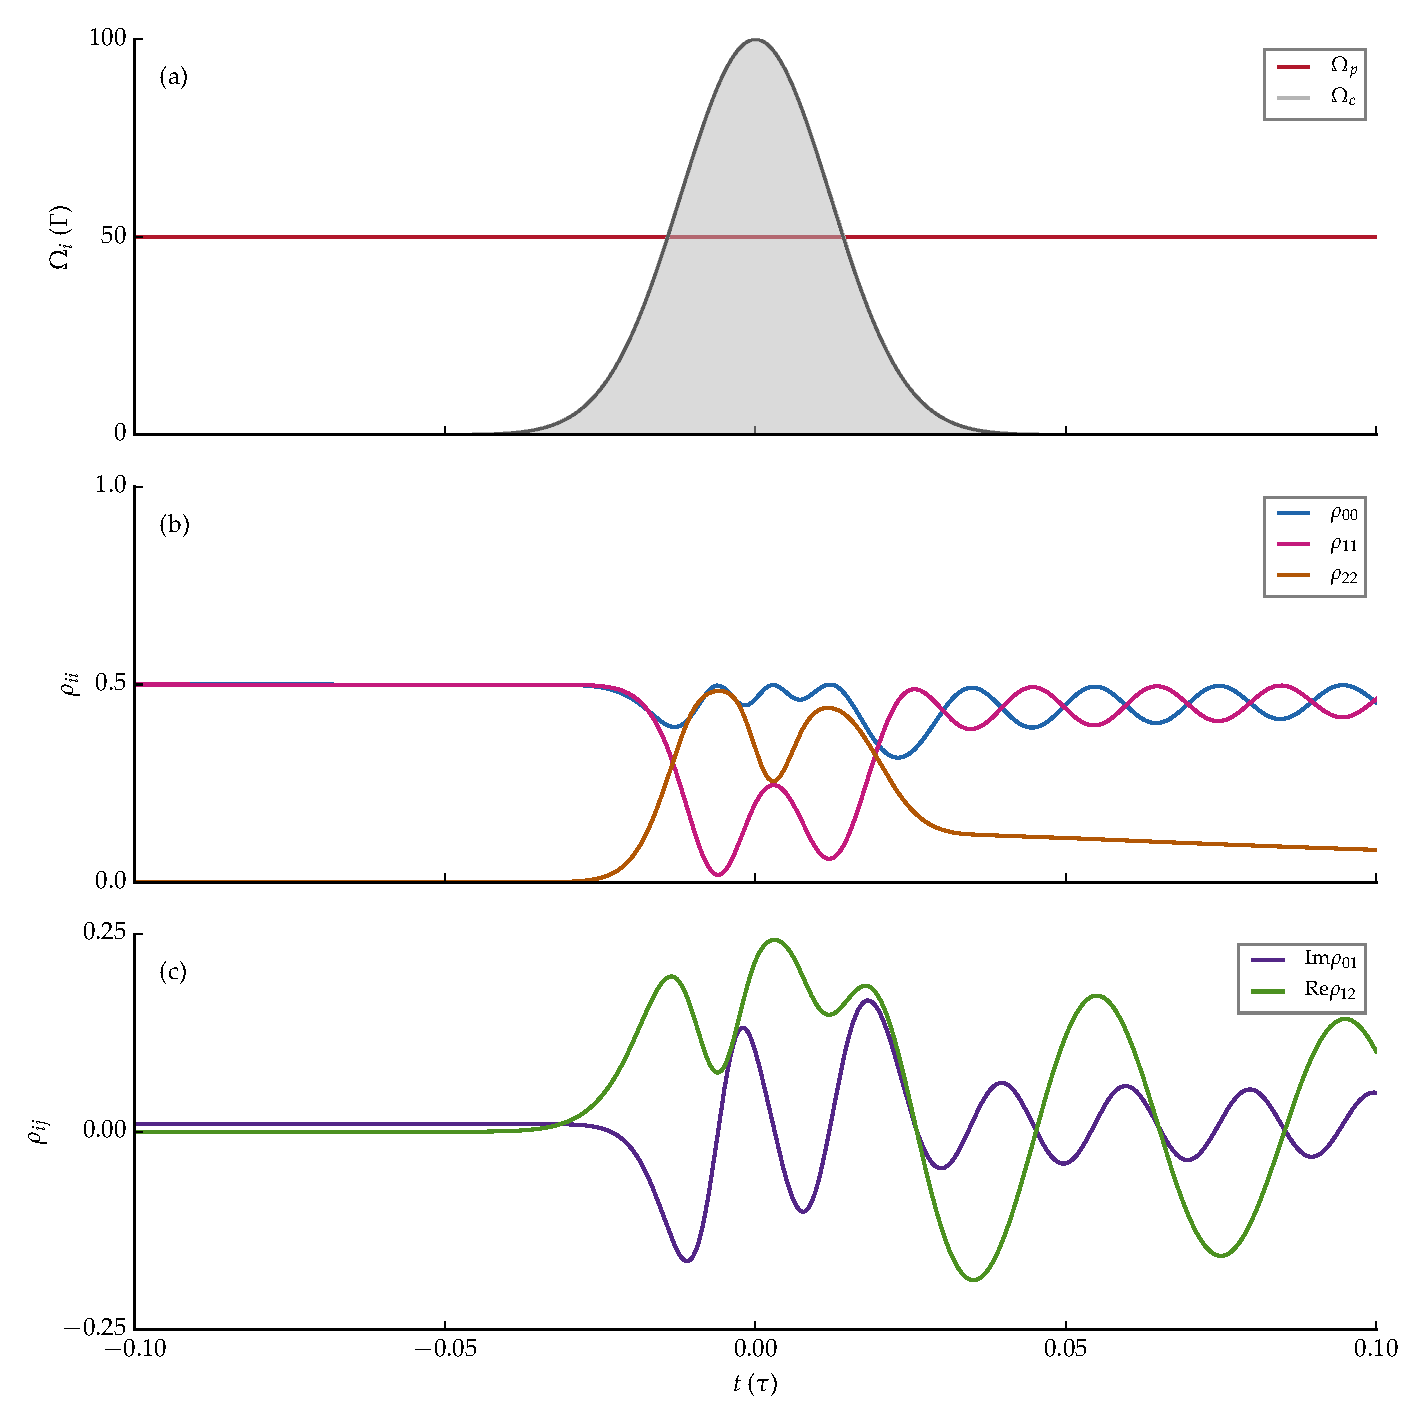
\includegraphics[width=\linewidth]{figs/06_simultons/ob_vee_solve_pls_t002_50c_100p_fig1.pdf}
    \caption{
    Time evolution of the density matrix elements from numerical solution of the
    master equation for the V configuration atom.  (a) Rabi frequency profiles
    of the two fields: a \textsc{cw} probe $\Omega_p$ (red) and Gaussian pulsed
    coupling $\Omega_c$ (grey) with amplitude $\unit[100]\Gamma$ and width $t_w
    = $ \unit[0.02]{$\tau_\Gamma$}. (b) Populations of the atomic eigenstates.
    (c) The imaginary part of coherence $\rho_{01}$ (purple) and the real part
    of coherence $\rho_{12}$ (green).
    }
    \label{fig:ob_vee_plse}
    \end{figure}

    In figure \ref{fig:ob_vee_plse} we show the time evolution of density matrix
    populations and coherences for an example Gaussian pulse profile of peak
    $\unit[100]\Gamma$ and width \unit[0.02]{$\tau_\Gamma$}, where here we'll
    assume $\Gamma := \Gamma_{01} = \Gamma_{02}$ and define $\tau_\Gamma :=
    \nicefrac{1}{\Gamma}$ as the reciprocal lifetime. The \textsc{cw} probe Rabi
    frequency is $\unit[50]\Gamma$. Before the pulse, the steady state
    population is an even split between $\rho_{00}$ and $\rho_{11}$. As the
    pulse ramps on we see it coherently drive population transfer such that it
    oscillates between populations $\rho_{11}$ and $\rho_{22}$. This is
    accompanied by a positive real coherence $\rho_{12}$, and an imaginary
    coherence $\rho_{01}$ which oscillates first negative and then positive.
    After the pulse we see damped oscillation of $\rho_{00}$ and $\rho_{11}$,
    and at long times we expect the system to return to its steady state.

    The behaviour of the imaginary part of $\rho_{01}$ is of particular interest
    as we know that the macroscopic consequence of this atomic coherence is
    polarisation of the medium with respect to the probe field, and resulting
    attenuation or amplification of that field. From the observed evolution we
    can then predict that during the pulse, without the populations $\Ket{0}$
    and $\Ket{1}$ being inverted, we will find reduced absorption and possibly
    gain in the probe field.

    To understand this time evolution, we write out the components of equation
    (\ref{eqn:lindblad}) for the V configuration to get a set of differential
    equations for the density matrix elements
    \begin{subequations}
    \begin{align}
    \frac{\partial \rho_{00}}{\partial t} &= \Gamma_{01} \rho_{11} + \Gamma_{02} 
    \rho_{22} + \frac{\ii}{2} \bigg[ \Omega_p 
    ( \rho_{01} - \rho_{10}) + \Omega_c ( \rho_{02} - \rho_{20}) \bigg] \\
    \frac{\partial \rho_{01}}{\partial t} &= -\frac{\Gamma_{01}}{2} \rho_{01} - 
    \ii \Delta_1 \rho_{01} + \frac{\ii}{2} \bigg[ \Omega_p 
    (\rho_{00} - \rho_{11}) - \Omega_c \rho_{21} \bigg] \\
    \frac{\partial \rho_{02}}{\partial t} &= -\frac{\Gamma_{02}}{2} \rho_{02} - 
    \ii \Delta_2 \rho_{02} + \frac{\ii}{2} \bigg[ -\Omega_p \rho_{12} + \Omega_c 
    ( \rho_{00} - \rho_{22} ) \bigg] \\
    \frac{\partial \rho_{11}}{\partial t} &= -\Gamma_{01} \rho_{11} - 
    \frac{\ii}{2} \Omega_p (\rho_{01} - \rho_{10}) \\
    \frac{\partial \rho_{12}}{\partial t} &= -\frac{\Gamma_{01}}{2} \rho_{12} - 
    \frac{\Gamma_{02}}{2} \rho_{12} + \ii (\Delta_1 - \Delta_2) \rho_{12} - 
    \frac{\ii}{2} (\Omega_p \rho_{02} - \Omega_c{\rho_{10}})\\
    \frac{\partial \rho_{22}}{\partial t} &= -\frac{\Gamma_{02}}{2} \rho_{22} - 
    \frac{\ii}{2} \Omega_c ( \rho_{02} - \rho_{20} ).
    \end{align}
    \label{eqn:vee_dm_equations}
    \end{subequations}
    Note that $\rho_{10} = \rho_{01}^\dagger$ and $\rho_{20} = \rho_{02}^\dagger$.


